\chapter{Esercizi di MR}
Svolgere gli esercizi nel seguente modo:
\begin{itemize}
    \item Identificare le relazioni che modellano il dominio descritto nel testo
    \item Identificare per ogni relazione le chiavi primarie e i vincoli di integrità referenziale
    \item Identificare almeno un vincolo di dominio
    \item Identificare quali attributi ammettono valori nulli
    \item Identificare un vincolo di ennupla
    \item Identificare una superchiave
    \item Identificare una chiave alternativa
\end{itemize}

\section{Es. A}
Si consideri il seguente schema di basi di dati che descrive un campionato provinciale di pallavolo. Le squadre si incontrano due volte, nel girone di andata e in quello di ritorno. Si tenga presente che il risultato di una partita di pallavolo è al meglio dei cinque set, non è detto che una squadra giochi le partite nella palestra dove si allena, più squadre possono allenarsi o giocare in giorni/orari diversi ma nella stessa palestra. 

\subsubsection{Identifico le relazioni: attributi}
\begin{itemize}
    \item SQUADRA (nome, capitano, città, palestraAll, cittàAll, palestraPart, cittàPart, sponsor)
    \item PALESTRA (nome, città, indirizzo, numPosti)
    \item ATLETA (tesserino, nome, cognome, dataNascita, luogoNascita, squadra)
    \item ARBITRO (tesserino, nome, cognome, dataNascita, luogoNascita, numPartiteArbitrate)
    \item SPONSOR (pIva, nome, telefono)
    \item RISULTATO (squadraCasa, squadraOspite, setSquadraCasa, setSquadraOspite, arbitro, palestra, città, data, oraInizio, oraFine)
\end{itemize}

\subsubsection{Identifico le chiavi primarie}
\begin{itemize}
    \item SQUADRA (\underline{nome}, capitano, città, \textbf{palestraAll}, cittàAll, palestraPart, cittàPart, sponsor)
    \item PALESTRA (\underline{nome, città}, indirizzo, numPosti)
    \item ATLETA (\underline{tesserino}, nome, cognome, dataNascita, luogoNascita, squadra)
    \item ARBITRO (\underline{tesserino}, nome, cognome, dataNascita, luogoNascita, numPartiteArbitrate)
    \item SPONSOR (\underline{pIva}, nome, telefono)
    \item RISULTATO (\underline{squadraCasa, squadraOspite}, setSquadraCasa, setSquadraOspite, arbitro, palestra, città, data, oraInizio, oraFine)
\end{itemize}

\subsubsection{Identifico gli attributi che possono essere nulli}
\begin{itemize}
    \item SQUADRA (nome, capitano, città, palestraAll, cittàAll, palestraPart, cittàPart, \textit{sponsor})
    \item PALESTRA (nome, città, indirizzo, numPosti)
    \item ATLETA (tesserino, nome, cognome, dataNascita, luogoNascita, squadra)
    \item ARBITRO (tesserino, nome, cognome, dataNascita, luogoNascita, \textit{numPartiteArbitrate})
    \item SPONSOR (pIva, nome, telefono)
    \item RISULTATO (squadraCasa, squadraOspite, \textit{setSquadraCasa, setSquadraOspite}, arbitro, palestra, città, data, oraInizio, oraFine)
\end{itemize}
\begin{center}
    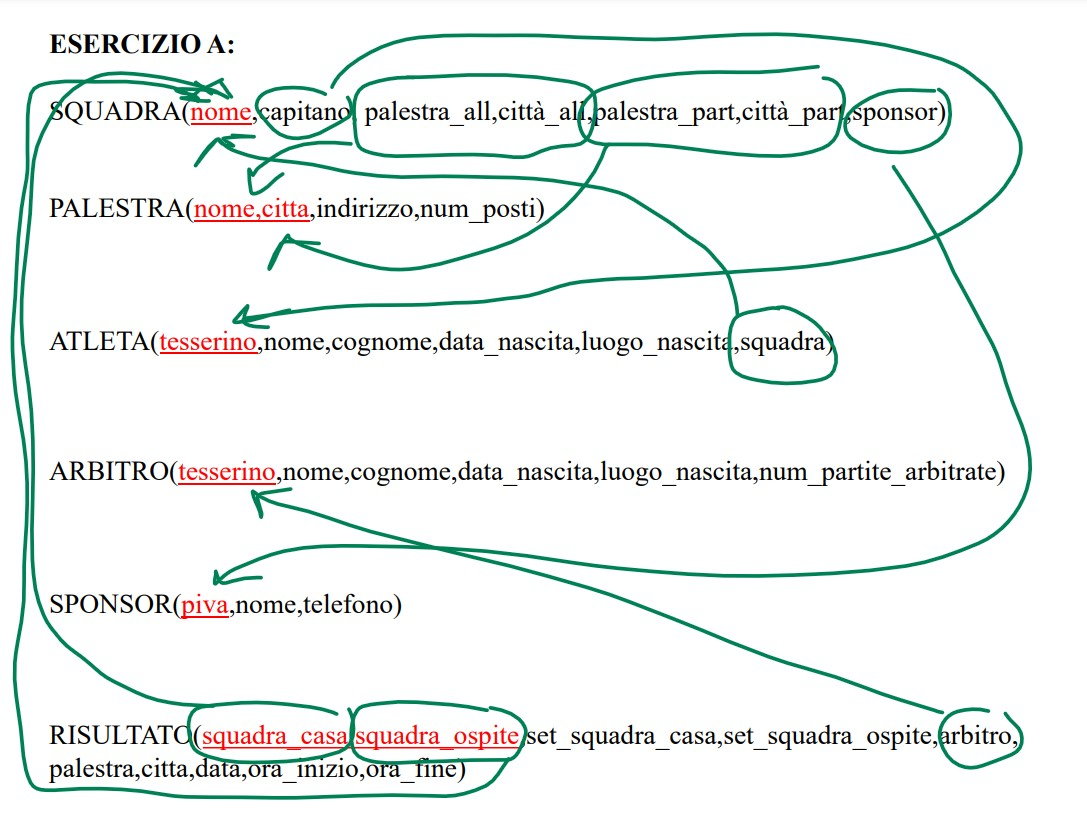
\includegraphics[width=0.675\textwidth]{chaptersLezioniSara/img/MR_fileesA.jpg}
\end{center}

\subsubsection{Identifico i vincoli di tupla}
\begin{itemize}
    \item setSquadraCasa e setSquadraOspite devono essere maggiori uguali di zero e minori uguali di 3.
    \item setSquadraCasa + setSquadraOspite deve essere maggiore uguale di 3 e minore uguale di 5.
    \item oraInizio < oraFine
    \item Una superchiave nella tabella sponsor è p.via, nome, telefono
    \item Una chiave alternativa è numTelefono in sponsor
\end{itemize}

\section{Es. B}
Si consideri il seguente schema di basi di dati che descrive le informazioni relative ad una olimpiade. Per ogni nazione si vuole tenere traccia dell'atleta porta bandiera, del numero di atleti, della mascotte e colore della divisa. Si vuole tenere traccia degli atleti e delle partecipazioni degli atleti alle gare con posizione raggiunta e fase della gara a cui sono arrivati. Per esempio nelle gare di corsa, le fasi possono essere: qualificazioni, ottavi, quarti, ecc. Ogni fase di gara ha due giudici e si svolgono ad una specifica data, ora e luogo. Per ogni atleta si vuole tenere traccia del codice tesserino atleta, nazione, cognome, nome e data di nascita.

\subsubsection{Identifico le relazioni}
\begin{itemize}
    \item NAZIONE (nome, portabandiera, numeroAtleti, mascotte, coloreDivisa)
    \item ATLETA (tesserino, nome, cognome, dataNascita, nazione)
    \item GARA (nomeGara, disciplina, recordMondiale, recordOlimpionico)
    \item SVOLGIMENTOGARA (gara, faseGara, luogo, data, ora, giudice1, giudice2)
    \item PARTECIPAZIONEGARA (atleta, gara, faseGara, posizioneClassifica, datiGara)
    \item GIUDICE (tesserino, nome, cognome, dataNascita, nazione)
\end{itemize}

\subsubsection{Identifico le chiavi primarie}
\begin{itemize}
    \item NAZIONE (\underline{nome}, portabandiera, numeroAtleti, mascotte, coloreDivisa)
    \item ATLETA (\underline{tesserino}, nome, cognome, dataNascita, nazione)
    \item GARA (\underline{nomeGara}, disciplina, recordMondiale, recordOlimpionico)
    \item SVOLGIMENTOGARA (gara, faseGara, luogo, data, ora, giudice1, giudice2)
    \item PARTECIPAZIONEGARA (atleta, gara, faseGara, posizioneClassifica, datiGara)
    \item GIUDICE (tesserino, nome, cognome, dataNascita, nazione)
\end{itemize}

\subsubsection{Identifico gli attributi che possono essere nulli}
Non è che abbia capito molto
\begin{itemize}
    \item NAZIONE (nome, portabandiera, numeroAtleti, mascotte, coloreDivisa)
    \item ATLETA (tesserino, nome, cognome, dataNascita, nazione)
    \item GARA (nomeGara, disciplina, recordMondiale, recordOlimpionico)
    \item SVOLGIMENTOGARA (gara, faseGara, luogo, data, ora, giudice1, \textbf{giudice2})
    \item PARTECIPAZIONEGARA (atleta, gara, faseGara, posizioneClassifica, datiGara)
    \item GIUDICE (tesserino, nome, cognome, dataNascita, nazione)
\end{itemize}
Boh da finire
\begin{center}
    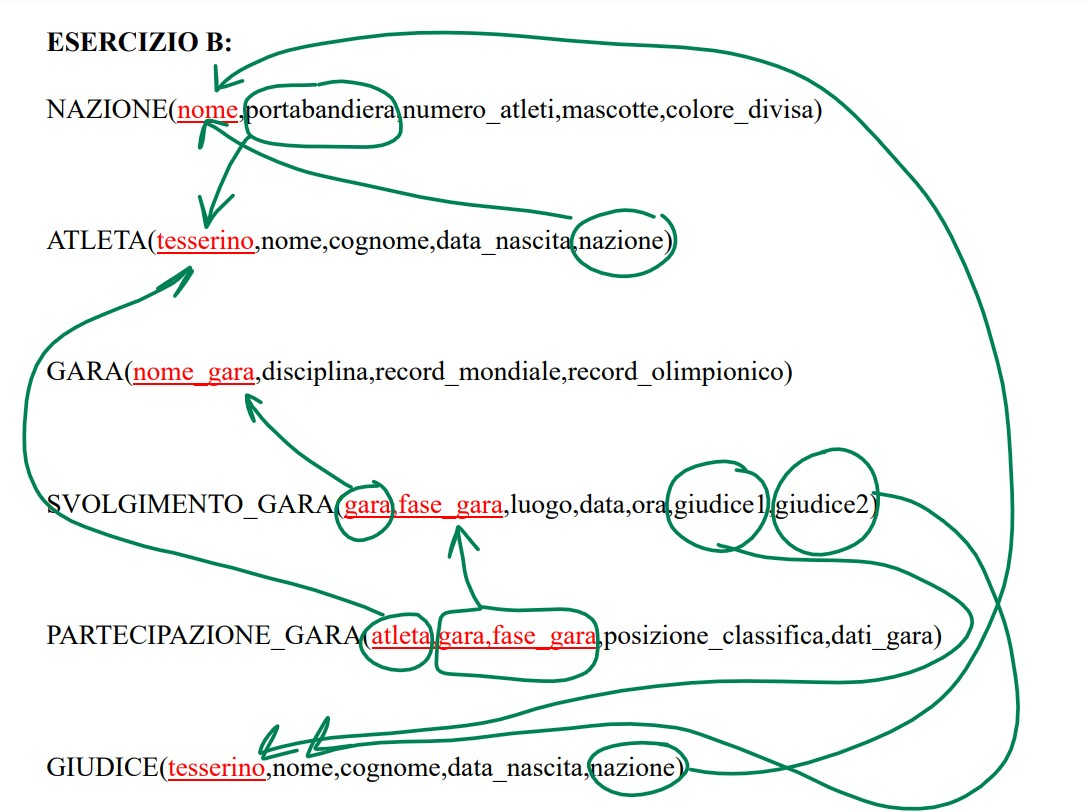
\includegraphics[width=0.675\textwidth]{chaptersLezioniSara/img/MR_fileesB.jpg}
\end{center}

\section{Es. C}
Si vuole rappresentare una base di dati relativa ai voli di una compagnia aerea. Si vuole tenere traccia dell'id del volo, del giorno della settimana, della città di partenza e di arrivo e ovviamente delle ore di partenza e arrivo. Un volo per esempio Milano-Parigi effettuato dall'aereo di tipo Airbus 300 che ha id=004 può essere svolto solo una volta durante una giornata. Per ogni tipologia di aereo si vuole tenere traccia del numero di passeggeri trasportabili, e quantità delle merci trasportabili. Ogni aeroporto è caratterizzato da una città, nazione e numero di piste. Si assuma la semplificazione che una città può avere un solo aeroporto.

\subsubsection{Identifico le relazioni}
\begin{itemize}
    \item AEROPORTO (Città, Nazione, NumPiste)
    \item AEREO (Tipo, NumPass, QuantMerci)
    \item VOLO (ID, Giorno, OraPart, OraArr, CittàPart, CittàArr, Aereo)
\end{itemize}

\subsubsection{Identifico le chiavi primarie}
\begin{itemize}
    \item AEROPORTO (\underline{Città}, Nazione, NumPiste)
    \item AEREO (\underline{Tipo}, NumPass, QuantMerci)
    \item VOLO (\underline{ID}, Giorno, OraPart, OraArr, CittàPart, CittàArr, Aereo)
\end{itemize}
\begin{center}
    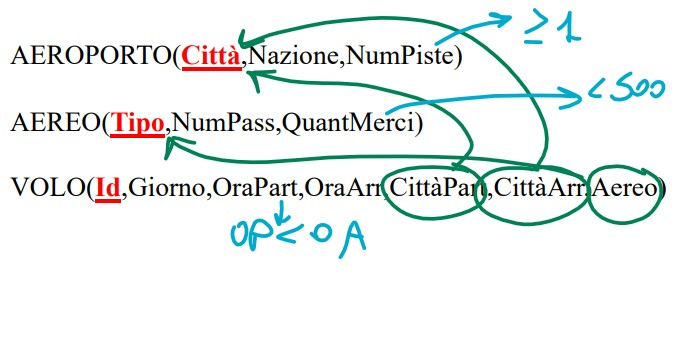
\includegraphics[width=0.675\textwidth]{chaptersLezioniSara/img/MR_fileesC.jpg}
\end{center}

\section{Es. D}
Si vuole rappresentare una base di dati relativa ai lavoratori delle aziende italiane. Per ogni lavoratore si vuole tenere traccia delle informazioni anagrafiche, delle città in cui ha abitato e lavorato e delle aziende in cui ha lavorato. Di ogni città si vuole conservare: nome, provincia e numero di abitanti. Per ogni azienda in cui le persone hanno lavorato si vuole tenere traccia del nome, P.IVA, città, numero impiegati e capitale sociale. Una azienda potrebbe aver nel tempo cambiato sede. Quindi ad esempio la Microsoft potrebbe avere avuto sede dal 1998 al 2009 a Rozzano e dal 2010 a Milano. Ogni lavoratore potrebbe aver lavorato in più aziende nel corso della sua vita.

\subsubsection{Identifico le relazioni: attributi}
\begin{itemize}
    \item PERSONA (CF, Nome, Cognome, DataNacita, CittàNascita)
    \item CITTA' (Codice, Nome, Provincia, NumAbitanti)
    \item AZIENDA (PIVA, Nome, Città, NumImpiegati, CapitaleSociale)
    \item ABITATO (Persona, Città, DataInizio, DataFine)
    \item LAVORATO (Persona, Azienda, Sede, DataInizio, DataFine)
    \item SEDE (CodiceSede, Azienda)
    \item LUOGOSEDE (CodiceSede, Città, Indirizzo, DataInizio, DataFine)
\end{itemize}
\begin{center}
    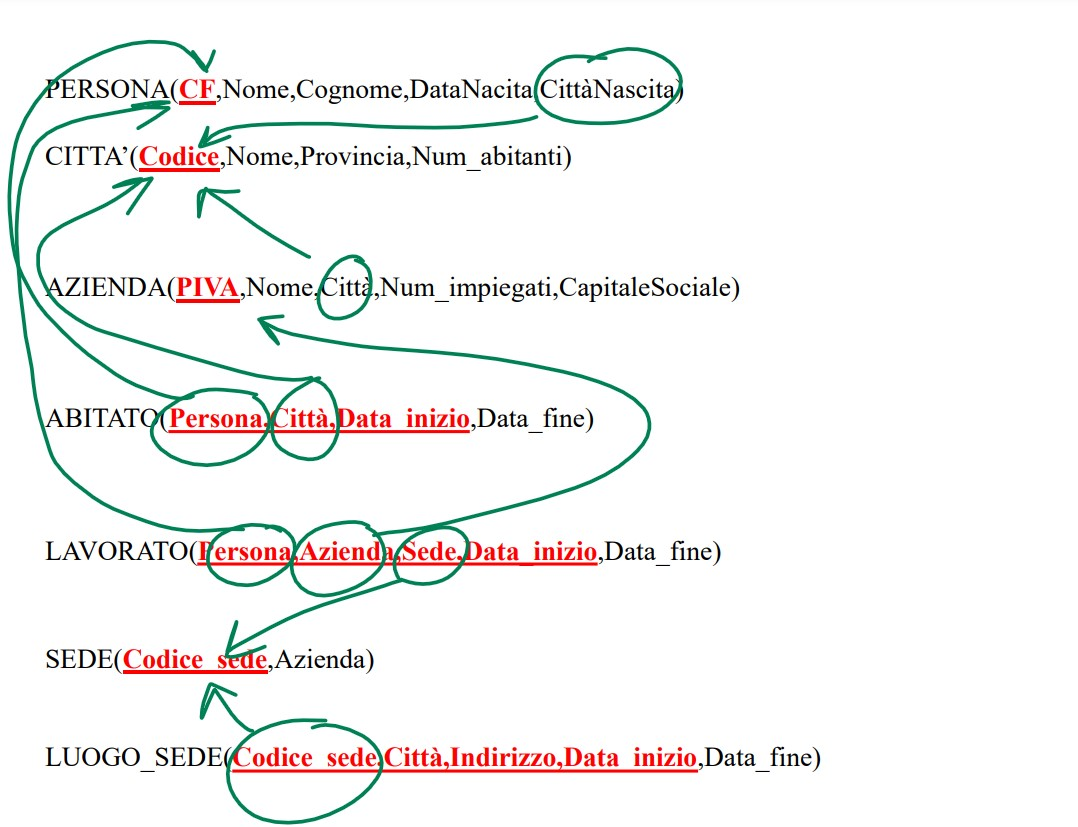
\includegraphics[width=0.675\textwidth]{chaptersLezioniSara/img/MR_fileesD.jpg}
\end{center}

\section{Es. E}
\section{Es. F}
\section{Es. G}